\documentclass[12pt]{article}
\usepackage[T1]{fontenc}
\usepackage[margin=2cm]{geometry}

\usepackage{amssymb}
\usepackage{amsmath}
\usepackage{tcolorbox}
\usepackage{xcolor}
\usepackage{framed}
\usepackage{euscript}
\usepackage{float}

\usepackage{verbatim}
\usepackage{mathrsfs}
\usepackage{graphicx}
\usepackage{multicol}

\usepackage{bbm,txfonts}
\usepackage{float}


\usepackage{titletoc}
\usepackage{tikz}
\usepackage{xspace}

\usepackage{enumitem}

\newcommand{\answer}{\vspace*{4pt} \noindent{\bf Solution: }}

\newcommand{\bb}[1]{\mathbb{#1}}
\renewcommand{\v}[1]{\boldsymbol{#1}}
\newcommand{\m}[1]{\mathbf{#1}}
\renewcommand{\c}[1]{\mathcal{#1}}
\usepackage{upquote}


\renewcommand{\tilde}{\widetilde}
\newcommand{\halmos}{\vspace{3mm} \hfill \mbox{$\Box$}}

\newcommand{\Var}{\mathbb{V}\mathrm{ar}}
\newcommand{\var}{\Var}

\newcommand{\Cov}{\mathbb{C}\mathrm{ov}}
\newcommand{\cov}{\Cov}

\renewcommand{\epsilon}{\varepsilon}
\renewcommand{\rho}{\varrho}
\renewcommand{\log}{\ln}
\renewcommand{\hat}{\widehat}

\newcommand{\iid}{\text{iid }}


% Bernoulli distribution
\newcommand{\Ber}{{\sf Ber}}
\newcommand{\ber}{\Ber}

% Binomial distribution
\newcommand{\Bin}{{\sf Bin}}
\newcommand{\bin}{\Bin}

% Cauchy distribution
\newcommand{\Cauchy}{{\sf Cauchy}}

% Negative binomial distribution
\newcommand{\NegBin}{{\sf NegBin}}

% Multinomial distribution
\newcommand{\Mnom}{{\sf Mnom}}
\newcommand{\mnom}{\Mnom}

% Geometric distribution
\newcommand{\Geo}{{\sf Geom}}
\newcommand{\geo}{\Geo}
\newcommand{\Geom}{\Geo}
\newcommand{\geom}{\Geo}
\newcommand{\G}{\Geo}

% Hypergeometric distribution
\newcommand{\Hyp}{{\sf Hyp}}

% Poisson distribution
\newcommand{\Poi}{{\sf Poi}}
\newcommand{\poi}{\Poi}
\newcommand{\Po}{\Poi}
\newcommand{\po}{\Poi}

% Uniform distribution (continuous)
\newcommand{\U}{\EuScript{U}}

% Exponential distribution
\newcommand{\Ex}{{\sf Exp}}
\newcommand{\ex}{\Ex}

% Normal / Gaussian distribution
\newcommand{\Nor}{\EuScript{N}}
\newcommand{\nor}{\Nor}

% Pareto distribution
\newcommand{\Pareto}{{\sf Pareto}}
\newcommand{\pareto}{\Pareto}

% Negative hypergeometric distribution
\newcommand{\NegHyp}{{\sf NegHyp}}

% Student's t distribution
\newcommand{\Student}{{\sf t}}
\newcommand{\student}{\Student}

% Gamma distribution
\newcommand{\Gam}{{\sf Gamma}}
\newcommand{\gam}{\Gam}

% Discrete uniform distribution
\newcommand{\DU}{{\sf DU}}

% Generic distribution
\newcommand{\Dist}{{\sf Dist}}

\newcommand{\Em}{{\mathbb E}}  % expectation
\newcommand{\Pm}{{\mathbb P}}  % probability measure
\newcommand{\R}{{\mathbb R}}

\newcommand{\gvn}{\,|\,}  % conditional (given)

\newcommand{\e}{\mathrm{e}} %Euler's e

\newcommand{\ds}{\displaystyle}

\newcommand{\di}{\mathrm{d}}  % use for differential symbol


\newcommand{\approxsim}{\stackrel{\mathrm{approx.}}{\sim}}

\newcommand{\iidsim}{\stackrel{\mathrm{iid}}{\sim}}
\newcommand{\simiid}{\iidsim}
\newcommand{\simiidt}{{\:{\sim}_{\mathrm{iid}}\:}}

%% Correlation
\newcommand{\Corr}{\mathrm{Corr}}
\newcommand{\corr}{\Corr}


\usepackage{cprotect}
\RequirePackage[formats]{listings}\RequirePackage{textcomp}

\lstnewenvironment{Pout}{%
  \lstset{backgroundcolor=\color{outcol},
  aboveskip= -2pt,  
  xleftmargin = 4pt,
  xrightmargin = 4pt,
  frame=single,
  upquote,
  framerule=1pt,
  basicstyle=\footnotesize\ttfamily,
  columns=fixed}}{}

%DK: See http://latexcolor.com/
\definecolor{applegreen}{rgb}{0.55, 0.41, 0.0}
\definecolor{gray1}{rgb}{0.98, 0.98, 0.98}
\definecolor{black}{rgb}{0, 0, 0}
\definecolor{cream}{rgb}{1.0, 0.99, 0.82}
\definecolor{islamicgreen}{rgb}{0.0, 0.56, 0.0}
\definecolor{vlgray}{gray}{0.9}
\definecolor{lgray}{gray}{0.7}
\definecolor{outcol}{gray}{0.9}

\tcbuselibrary{listings,skins,breakable,theorems}

\newenvironment{PC}{%
\tcblisting{breakable,listing only,colback=cream, enhanced, sharpish
corners,  boxrule=1pt,after, listing options =
   {language=Python,
  basicstyle=\footnotesize\ttfamily,        % the size of the fonts that are used for the code
  numbers=none,                   % where to put the line-numbers
%  numberstyle=\tiny\color{blue},  % the style that is used for the line-numbers
  xleftmargin=-10pt,
  aboveskip=-4pt,
  belowskip=-6pt,
  columns=fixed,
  basewidth=5pt,                     %separation of letters
%  stepnumber=1,                % the step between two line-numbers. If it's 1, each line will be numbered
%  numbersep=7pt,                  % how far the line-numbers are from the code
  backgroundcolor=\color{cream},  % choose the background color. You must add \usepackage{color}
  showspaces=false,               % show spaces adding particular underscores
  showstringspaces=false,         % underline spaces within strings
  showtabs=false,                 % show tabs within strings adding particular underscores
  %frame=single,                   % adds a frame around the code
  %frame=shadowbox,
  %rulecolor=\color{black},        % if not set, the frame-color may be changed on line-breaks within not-black text (e.g. comments (green here))
  tabsize=2,                     % sets default tabsize to 2 spaces
 % captionpos=b,                  % sets the caption-position to bottom
  breaklines=true,                % sets automatic line breaking
  breakatwhitespace=false,        % sets if automatic breaks should only happen at whitespace
  %title=\lstname,                 % show the filename of files included with \lstinputlisting;
                                  % also try caption instead of title
  keywordstyle=\color{blue},      % keyword style
  upquote,     % very important to get right quote for cut/paste
  commentstyle=\color{islamicgreen},   % comment style
  stringstyle=\color{red},      % string literal style
 % escapeinside={\%*}{*)},         % if you want to add a comment within your code
  morekeywords={*,...}
  			 }
    		}
    	}
{\endtcblisting}






\usepackage{url}
\usepackage{fancyhdr}
\usepackage{natbib}
\usepackage{fvextra}
\usepackage{tikz}
\usetikzlibrary{shapes.geometric, arrows.meta, positioning, fit, backgrounds}
\DefineVerbatimEnvironment{Code}{Verbatim}{
    fontsize=\footnotesize, % Adjust font size
    breaklines=true,        % Enable line wrapping
    breakanywhere=true      % Allow breaking anywhere
}

% \title{Statistical Arbitrage and Deep Learning in the European Electricity Market \\ Deep Learning (STAT3007/7007) \\ Report - Semester 1, 2025.}

\title{Integrating Weather Data into Deep Learning-Based Statistical Arbitrage \\ Deep Learning (STAT3007/7007) \\ Report - Semester 1, 2025.}

\author{\normalsize
    Filip Orestav\\ \normalsize
    49316997
    \and \normalsize
    Hans Stemshaug\\ \normalsize
    49060423
    \and \normalsize
    Nila Saravana\\ \normalsize
    48773799
    \and \normalsize
    Volter Entoma\\ \normalsize
    44782711
    \and \normalsize
    Weiming Liang\\ \normalsize
    46375489
}

\begin{document}

\maketitle

%%%%%%%%%%%%%%%%%%%%%%%%%%%%%%%%%%%%%%%%

% Introduction

%%%%%%%%%%%%%%%%%%%%%%%%%%%%%%%%%%%%%%%%

\section{Introduction}

Statistical Arbitrage is a trading strategy that aims to profit from the relative price movements of two or more assets.  It involves identifying mispricings in the market and taking advantage of them by simultaneously buying and selling the assets. Statistical arbitrage is based on the idea that pairs or groups of historically similar stocks are expected to maintain their statistical relationship in the future, allowing traders to exploit temporary deviations from this relationship. \citep{avellaneda2010statistical}

The goal for this project is to develop a deep learning model that can apply Statistical Arbitrage to identify unfairly priced electricity prices in the European market, and to create a profitable trading strategy.

\clearpage

%%%%%%%%%%%%%%%%%%%%%%%%%%%%%%%%%%%%%%%%

% Literature Review

%%%%%%%%%%%%%%%%%%%%%%%%%%%%%%%%%%%%%%%%

\section{Literature Review}

\citep{guijarro2021deep}






\begin{itemize}
    \item There model we use in this report
        \begin{itemize}
            \item Architecture design: what are the components, the purpose of their components 
            \item Main findings of the paper and how that's relevant to our current study 
            \item Insert a figure of their architecture
            \item Discuss which part of their model and we're going to use and why
        \end{itemize}
    \item https://ieeexplore.ieee.org/abstract/document/9383387
"Electricity price forecast based on weekly weather forecast and its application to arbitrage in the forward market" (This paper should have something about how weather affects the supply and demand of electricity and hence the prices)
    \item success stories of incorporating different data source into statistical arbitrage and get good results 
\end{itemize}



\clearpage

%%%%%%%%%%%%%%%%%%%%%%%%%%%%%%%%%%%%%%%%

% Theory

%%%%%%%%%%%%%%%%%%%%%%%%%%%%%%%%%%%%%%%%

\section{Theory}

\subsection{Long-Short Portfolio}
A long-short portfolio is a trading strategy that involves taking long positions in undervalued assets and short positions in overvalued assets. The goal of this strategy is to profit from relative movement of an asset relative to others within the portfolio. 
Going \textbf{long} on an asset means buying the asset with the expectation that its price will increase, allowing the trader to sell it later at a higher price. Conversely, going \textbf{short} on an asset means borrowing the asset and selling it with the expectation that its price will decrease, allowing the trader to buy it back later at a lower price and return it to the lender.

\vspace{10pt}
\noindent
The long-short portfolio is constructed such that the total value of the long positions is equal to the total value of the short positions, allowing the trader to profit from the movements of assets relative to the other assets within the portfolio, rather than from the overall market movement.

\subsection{Statistical Arbitrage: Cointegration}

Cointegration is a statistical property of a set time series variables that indicates a long-term correlation between them. The basis of cointegration is that historically correlated time series can deviate from their correlation in the short term, but will eventually revert to being correlated.

\vspace{10pt}
\noindent
Consider $N$ assets with log cumulative returns $R_{1,t}, R_{2,t}, \ldots, R_{N,t}$. We can investigate wether the time series of the first asset $R_{1,t}$ is correlated with the time series of all the other assets $R_{2,t}, \ldots, R_{N,t}$ by looking at the residuals of the first asset after regressing it on the other assets.

\begin{equation}
\epsilon_{1,t} = R_{1,t} - \sum_{i=2}^{N} \beta_{1,i} R_{i,t}
\label{eq:cointegration_single}
\end{equation}

\noindent
The residual $\epsilon_{1,t}$ is the difference between the log cumulative return of the first asset and a linear combination of the log cumulative returns of the other assets, at time $t$. If this residual centers around a constant mean (typically at zero), it indicates that the first asset is \textbf{cointegrated} with the other assets.

\noindent
We can extend this idea for all $N$ assets, by looking at the residuals of each asset after regressing it on all the other assets. If the residuals of all the assets center around a constant mean, it indicates that all the assets are cointegrated with each other.

\begin{equation}
\epsilon_{n,t} = R_{n,t} - \sum_{j=1, j \neq n}^{N} \beta_{n,j} R_{j,t}
\label{eq:cointegration_all}
\end{equation}

\noindent
Where $\epsilon_{n,t}$ is the residual of asset $n$ at time $t$, and $\beta_{n,j}$ is the coefficient of asset $j$ in the regression of asset $n$ on all the other assets. 

\vspace{10pt}
\noindent
The signficance of cointegration is that it allows us to determine whether an asset is undervalued or overvalued relative to the other assets. If the residuals of an asset deviate significantly from zero, it indicates that the asset is either undervalued or overvalued relative to the other assets. This allows traders to take advantage of these deviations by taking long or short positions in the assets.

\begin{itemize}
  \item \textbf{Long} the undervalued assets.
  \item \textbf{Short} the overvalued assets.
\end{itemize}

\vspace{10pt}
\noindent
For example, if $e_{i,t} > 0$, it indicates that asset $i$ is overvalued. Traders would short the asset. Conversely, if $e_{i,t} < 0$, it indicates that asset $i$ is undervalued, and traders would go long on the asset.

\vspace{10pt}
\noindent
In Equation~\ref{eq:cointegration_all}, it is up to the user to choose the length and time period of the cointegration. For the rest of the report, we refer to a particular period of cointegration as a \textbf{cointegration window}. The length of the cointegration window is the number of days used to calculate the residuals, and the time period is the start and end date of the cointegration window.
When picking the length of the cointegration window is a trade-off between capturing long-term trends and short-term fluctiations. A longer cointegration windows allows for a more comprehsive cointegration, however, it sacrifices the ability to capture short-term trends. A shorter cointegration window allows for a more responsive model, however, it sacrifices the ability to capture long-term trends. The choice of the length of the cointegration window is a trade-off between these two extremes - for this report, we will use a cointegration window of 365 days. However, this choice is largely arbitrary, and the performance of the model may vary depending on the length of the cointegration window.  

\vspace{10pt}
\noindent
In the context of European electricity prices, we expect the prices in Europe to be highly correlated, as there are balancing effects of supply and demand. Many European countries are connected via cross-border transmission lines, allowing to equalize prices across interconnected countries. Additionally, neighbouring regions are expected to experience similar weather patterns, and seasonal demand, leading to correlated markets. Lastly, European energy policies and regulations are often harmonzied, reducing energy structural difference between countries.

\subsubsection{Log returns}

We take the log of the cumulative returns of the time series for each asset. This is done to capture any compounding differences between the assets and stabilizes large variances. Additionally, taking the cumulative returns instead of the raw prices allows us to capture the relative change in price over time, normalizing the data and making it easier to compare across different assets. Cointegration between log returns is more likely to be stationary than cointegration between raw prices.

\vspace{10pt}
\noindent
Specifically, the log return of asset $n$ at time $t$:

\begin{equation}
    R_{i,t} = \log\left( \frac{P_{i,t}}{P_{i,0}} \right)
    \label{eq:log_cumulative_return}
\end{equation}

\noindent
Where $P_{i,t}$ is the price of asset $i$ at time $t$ and $P_{i,0}$ is the price of asset $i$ at time $0$. The log return is a measure of the relative change in price over time.

\noindent
We can simply this by defining the vector $\mathbf{R}_t$ as the vector of log cumulative returns for all assets at time $t$, and the vector $\mathbf{P}_t$ as the vector of prices for all assets at time $t$. The log cumulative return vector is then defined as:

\begin{equation}
    \mathbf{R}_t = \log\left( \frac{\mathbf{P}_t}{\mathbf{P}_0} \right)
    \label{eq:log_cumulative_return_vector}
\end{equation}

\subsubsection{Cumulative residuals}

The cumulative sum mimics a \textit{price-like} behavior, which is more suitable for identifying trading signals. (\textcolor{red}{Needs citation here}) Raw residuals may not capture sufficient trend information, while cumulative forms highlight \textit{deviations} more clearly.

\vspace{10pt}
\noindent
The cumulative residuals are calculated by integrating the time series of residuals over a window from day $t_{i}$ to $t_{f}$. For asset $n$, define $\epsilon^{t_i,t_f}_{n,t}$ as the vector of the past residuals from day $t_{i}$ to day $t_{f}$:
\begin{equation}
    \mathbf{\epsilon}^{t_i,t_f}_{n,t} = \left( \epsilon_{n,t_i},\ \epsilon_{n,t_i+1},\ \ldots,\ \epsilon_{n,t_f} \right)
    \label{eq:residual_vector}
\end{equation}

\noindent
The \textbf{cumulative residual vector} $\mathbf{x}_n^{t_i, t_f}$ is then defined as:
\begin{equation}
    \mathbf{x}_{t_i,t_f}^{(n)} := \mathrm{Int}(\epsilon^{t_i, t_f}_{n,t}) 
      = \left( \mathbf{\epsilon}_{n,t_i},\ \mathbf{\epsilon}_{n,t_i} + \mathbf{\epsilon}_{n,t_i+1},\ \mathbf{\epsilon}_{n,t_i} + \mathbf{\epsilon}_{n,t_i+1} + \mathbf{\epsilon}_{n,t_i+2},\ \ldots,\ \sum_{t=t_i}^{t_f} \mathbf{\epsilon}_{n,t} \right)
    \label{eq:cumulative_residual}
\end{equation}

\noindent
Where $\mathrm{Int}$ is the integration operator, and $\mathbf{\epsilon}_{n,t}$ is the residual of asset $n$ at time $t$. For the rest of the report, we will refer to the period from $t_i$ to $t_f$ as the \textbf{cumulative residual window}.

\vspace{10pt}
\noindent
This report arbitrarily uses the cumulative residual window size of $L=t_f-t_i=30$ days. We expect that the choice of $L$ would affect the performance of the model, however, exploring different values of $L$ is out of the scope of this project.

\subsubsection{Portfolio positions}

For this report, we define a portfolio position as a vector $w$ of weights for each asset in the portfolio. The weights represent the long or short position of each asset in the portfolio, and are soft normalized such that they sum to 1. The portfolio position is defined as:

\begin{equation}
    \mathbf{w} = (w_1, w_2, \ldots, w_N)
    \label{eq:portfolio_weights}
\end{equation}

\noindent
Where $w_i$ is the weight of asset $i$ in the portfolio. The weights are soft normalized such that:

\begin{equation}
    \sum_{i=1}^{N} w_i = 1
    \label{eq:portfolio_weights_normalization}
\end{equation}

\subsubsection{Model performance evaluation} 

\subsubsection*{Returns}

Given the portfolio position $\mathbf{w}_t$ at time $t$, the return of the portfolio at time $t$ is defined as the matrix product of the portfolio weights and the vector of log returns of all assets at time $t+1$. The return is defined as:

\begin{equation}
    \mathbf{r}_t = \mathbf{w}_t^\top \mathbf{R}_{t+1}
    \label{eq:returns}
\end{equation}

\noindent
Where $R_{t+1}$ is the vector of log returns for all assets at time $t+1$, and $w$ is the vector of portfolio weights at time $t$. 

\subsubsection*{Sharpe ratio}

The Sharpe ratio (SR) is a measure of risk-adjusted return, calculated as the ratio of the mean excess return and the standard deviation of the excess return. It is used to evaluate the performance of a trading strategy or investment portfolio. A higher Sharpe ratio indicates better risk-adjusted performance. Therefore, we use the negative of the Sharpe ratio as the loss function for our model. 

\vspace{10pt}
\noindent
Consider the set of returns $\mathbf{r} = (r_1, r_2, \ldots, r_T)$, where $T$ is the number of returns. The Sharpe ratio is calculated as:

\begin{equation}
    \text{SR} = \frac{\mathbb{E}[\mathbf{r}]}{\text{Std}[\mathbf{r}]}    
    \label{eq:sharpe_ratio}
\end{equation}

\noindent
Where $\mathbb{E}[\mathbf{r}]$ is the mean of the returns, and $\text{Std}[\mathbf{r}]$ is the standard deviation of the returns. The negative of this Sharpe ratio is then used as the loss function for the model.

\clearpage



%%%%%%%%%%%%%%%%%%%%%%%%%%%%%%%%%%%%%%%%

% Data

%%%%%%%%%%%%%%%%%%%%%%%%%%%%%%%%%%%%%%%%

\section{Data}

We have two different datasets. One containing the electricity prices for 31 different countries in Europe, and a second dataset containing weather data for these countries, in the same period. 

\subsection{European electricity prices}

The electricity price data used in this project was taken from EMBER's \textit{European Wholesale Electricity Price Data} \citep{ember2025}.  The data used in this report consists of daily electricity prices for 31 European countries from 2015 to 2025. The data was downloaded in CSV format and preprocessed to remove any missing values. The information contained in the dataset is the country, data, and price given in EUR per MWh. 

\subsection{European weather data}
We used the dataset \textit{ERA5 hourly time-series data on single levels from 1940 to present}. \citep{hersbach2025era5}. This data originally contained hourly weather data, such as wind speed, precipitation and temperature above 2m above sea level. For us to use this dataset, we have aggregated the data to daily instead of hourly. For each of the data columns, we have taken the average during the day, aswell as the maximum and minimum values. 

Now Filip will talk about the model and training workflow

% \begin{itemize}
%     \item What is a available in the dataset? What and how did we extract the information we need? How did we preprocess the data?
% \end{itemize}

 \clearpage

%%%%%%%%%%%%%%%%%%%%%%%%%%%%%%%%%%%%%%%%

% Models

%%%%%%%%%%%%%%%%%%%%%%%%%%%%%%%%%%%%%%%%

\section{Models}
\subsection*{Input Preperation}

We prepare the input data for the model using the following steps:

\subsubsection*{Create cointegration windows:}
\begin{itemize}
    \item The full historical dataset (2015–2024) is segmented into \textbf{cointegration windows} of 365 days, rolling forward every 182 days.
\end{itemize}

\subsubsection*{Within each cointegration window:}

\begin{enumerate}
    \item \textbf{Log Cumulative Returns}:
    \begin{itemize}
        \item For each asset $n$, calculate the log cumulative returns as defined in Equation~\eqref{eq:log_cumulative_return}.
        \item Shapes:
        \begin{itemize}
            \item Input price matrix: $P \in \mathbb{R}^{N \times T}$
            \item Output return matrix: $R \in \mathbb{R}^{N \times T}$
        \end{itemize}
    \end{itemize}

    \item \textbf{Cointegration Residuals}:
    \begin{itemize}
        \item Compute residuals by regressing each asset’s returns on all others, as defined in Equation~\eqref{eq:cointegration_all}.
        \item Output shape: $\varepsilon \in \mathbb{R}^{N \times T}$
    \end{itemize}

    \item \textbf{Cumulative Residuals (Window Length $L = 30$)}:
    \begin{itemize}
        \item Within each cointegration window, we slide a fixed-length window of 30 days across time \textbf{one day at a time} to construct the model input.
        
        \item For each starting index $t_i$, we compute a sequence of cumulative sums over the next 30 days, as defined in Equation~\eqref{eq:cumulative_residual}:

                \item One input to the model:
        \[
        \mathbf{x} \in \mathbb{R}^{N \times L}
        \quad \text{(cumulative residuals across $N$ assets and $L = 30$ days)}
        \]

        \item If weather data is used, it is concatenated channel-wise:
        \[
        \mathbf{x}_{\text{aug}} \in \mathbb{R}^{(N + W) \times L}
        \]
        where $W$ is the number of weather features (e.g., temperature, wind, precipitation).
    \end{itemize}

    \item \textbf{Next-Day Return Target}:
    \begin{itemize}
        \item For each residual window ending at day $t$, define the next-day return target as:
        \[
        \mathbf{y}_t = \mathbf{R}_{t+1} \in \mathbb{R}^N
        \]
        where $\mathbf{R}_{t+1}$ is defined by Equation~\eqref{eq:log_cumulative_return_vector}.
    \end{itemize}
\end{enumerate}

\subsection*{Architecture:}
\begin{itemize}
    \item CNN+(Transforer)+FFN
    \item 2 Layers of CNN 1D with RELU Activation
    \item Transformer component in the  (can be turned off)
    \item FFN which ouput the learned underlying feature of the data into a vector the same size of the number of countries in the dataset, and soft normalised for constructing the portfolio.
\end{itemize}

\begin{table}[htpb]
    \centering
    \begin{tabular}{c|c}
        Data & Architecture \\ 
        \hline \hline 
        Price Data Only & CNN + FNN \\ 
        Price Data + Weather Data & CNN + FNN \\ 
        Price Data Only & CNN + Transformer + FNN \\ 
        Price Data + Weather Data & CNN + Transformer + FNN \\
        \hline \hline 
    \end{tabular}
    \caption{Caption}
    \label{tab:my_label}
\end{table}

\subsection*{Model Outputs}

For every input, the model outputs a vector of portfolio weights $w$ for each asset, using Equation~\ref{eq:portfolio_weights}. The output is a soft normalized vector of the portfolio positions, where each value represents the weight of the corresponding asset in the portfolio. The weights are normalized such that they sum to 1, and they are constrained to be between -1 and 1. This means that the model can take long or short positions in each asset, but the total position in each asset is limited to 100\% of the portfolio value. 
\\

These weights are then multiplied by the price of the assets one day after the end of the associated input's cumulative residual window. This gives the model's next-day return for that input.
\\

The set of inputs creates a set of next-day returns, which are then used to calculate the Sharpe ratio of the model's performance for that cointegration period. The Sharpe ratio is calculated using Equation~\ref{eq:sharpe_ratio}, and the negative of the Sharpe ratio is used as the loss function for the model.

% \subsection{CNN+Tranformer+FFN}

\clearpage

%%%%%%%%%%%%%%%%%%%%%%%%%%%%%%%%%%%%%%%%

% Results

%%%%%%%%%%%%%%%%%%%%%%%%%%%%%%%%%%%%%%%%

\section{Results}

\clearpage

%%%%%%%%%%%%%%%%%%%%%%%%%%%%%%%%%%%%%%%%

% Discussion

%%%%%%%%%%%%%%%%%%%%%%%%%%%%%%%%%%%%%%%%


\section{Discussion}
\clearpage
%%%%%%%%%%%%%%%%%%%%%%%%%%%%%%%%%%%%%%%%

% References

%%%%%%%%%%%%%%%%%%%%%%%%%%%%%%%%%%%%%%%%


\bibliographystyle{apalike}
\bibliography{references.bib}

\clearpage

\section{Appendix}
% Input figure of input preparation pipeline
\begin{figure}[H]
    \centering
    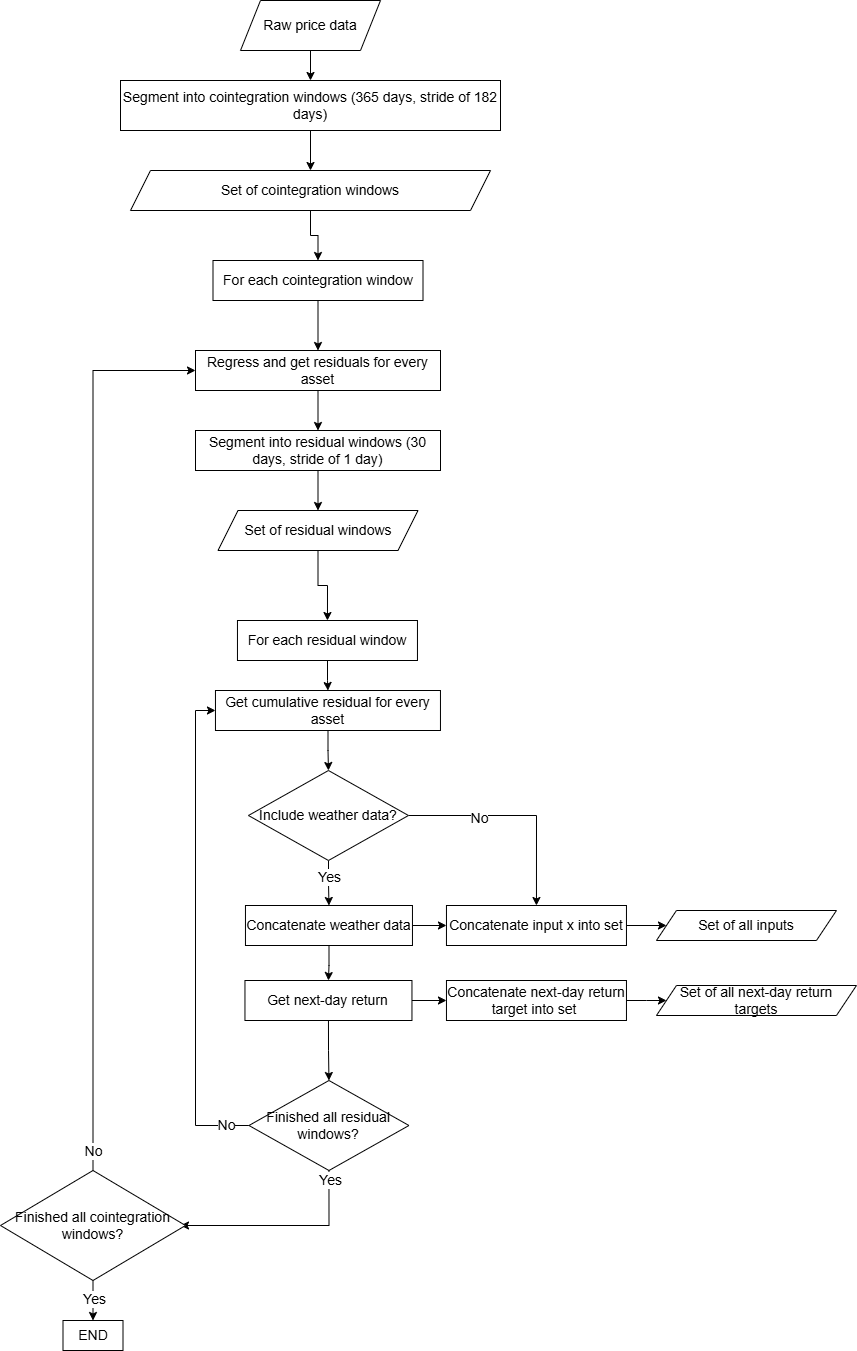
\includegraphics[width=0.8\textwidth]{figures/input_preparation_pipeline.drawio.png}
    \caption{Input Preparation Pipeline for Deep Learning Model}
    \label{fig:input_preparation_pipeline}
\end{figure}

\clearpage

\end{document}
